\documentclass[UTF8, fontset=mac]{ctexart}

\usepackage{latexsym}
\usepackage[empty]{fullpage}
\usepackage{titlesec}
\usepackage{marvosym}
\usepackage[usenames,dvipsnames]{color}
\usepackage{verbatim}
\usepackage{enumitem}
\usepackage[hidelinks]{hyperref}
\usepackage{fancyhdr}
\usepackage{graphicx}  % 用于包含图像
\usepackage{wrapfig}   % 用于图像的文本环绕效果
\usepackage{fontspec}
\usepackage{ctex}
\usepackage{ifthen}
\usepackage{etoolbox}
\usepackage{stmaryrd}
\usepackage{xcolor}
\usepackage{textcase}
\usepackage{tikz}

\newfontfamily\allcapfont{Arsenal SC}
\newfontfamily\allcapfontb{Alegreya SC}
\newfontfamily\namefont{Baskervville SC}


\newcommand{\CAP}[1]{\allcapfont #1}
\newcommand{\dashedhline}{ %
\vspace{-12pt}
\noindent
  \tikz[baseline]{%        % wrap the whole picture in braces
    \draw[dashed,gray,line width=.5pt] (0,0) -- (\linewidth,0);%
  }%                       % picture ends
\vspace{-25pt}
}%

\definecolor{Icon}{RGB}{243,182,0}
\definecolor{TextHighlight}{RGB}{162, 122, 0}
\definecolor{Text}{RGB}{60, 60, 60}
\definecolor{icon}{RGB}{100, 100, 100}
\definecolor{Accent}{RGB}{0, 0, 0}
\AtBeginDocument{\color{Text}}

% then load xeCJK (or luaCJK)            % for XeLaTeX; replace with luaCJK for LuaLaTeX
% set your CJK (Chinese) fonts:
\setCJKmainfont   {Songti SC}      % (macOS) 思源宋体
\setCJKsansfont   {Heiti SC}       % (macOS) 思源黑体
\setCJKmonofont   {Songti SC}    % or another monospace you have

% set your CJK (Chinese) fonts:

\usepackage{fontawesome5}
\newcommand{\Icon}[1]{{\color{Icon}\faIcon{#1}\,~}}  % helper macro
\newcommand{\icon}[1]{{\color{icon}\faIcon{#1}\,~}}  % helper macro
\newcommand{\HugeName}{\fontsize{38pt}{21.6pt}\selectfont \namefont}
\newcommand{\link}[2]{\href{#1}{\underline{\textbf{#2}}}}
\setmainfont{Times New Roman}        % 宋体
%\usepackage{newtxtext,newtxmath}
\pagestyle{fancy}
\fancyhf{} % clear all header and footer fields
\fancyfoot{}
\renewcommand{\headrulewidth}{0pt}
\renewcommand{\footrulewidth}{0pt}

% Adjust margins
\addtolength{\oddsidemargin}{-0.530in}
\addtolength{\evensidemargin}{-0.375in}
\addtolength{\textwidth}{1in}
\addtolength{\topmargin}{-.45in}
\addtolength{\textheight}{1in}
\setlength{\footskip}{3.60004pt}

\raggedbottom
\raggedright
\setlength{\tabcolsep}{0in}

% Sections formatting
\titleformat{\section}{
    \vspace{-10pt}\raggedright\large
}{}{0em}{}[{\color{Icon}\titlerule[1.5pt] \vspace{-6pt}}]

%------------------------------------------------------
% Language mode switch: set one of these.
%\newif\ifEnglish
%\Englishtrue    % Uncomment for English output.
%%\Englishfalse   % Uncomment for Chinese output.
% Check the value of \LanguageMode


% Command to choose the language: first argument = English, second = Chinese.
\newcommand{\lang}[2]{\ifEnglish #1\else #2\fi}
\newcommand{\pill}[1]{%
    \tikz[baseline={(X.base)}]
    \node[
        draw=Icon,
        line width=0.8pt,         % increased border weight
        rounded corners=4pt,     % make the corners rounded
        inner xsep=6pt,          % horizontal padding
        inner ysep=2pt           % vertical padding
    ] (X) {\texttt{#1}};%
}

% Custom commands for bilingual CV components:
\newcommand{\cvsection}[3]{\section{
    \Icon{#3}{\Large\color{TextHighlight}\lang{\CAP{#1}}{#2}}
}}

% The subheading command takes 6 arguments:
% 1: Title, 2: Institution, 3: Location,
% 4: Role/Detail, 5: Supervisor, 6: Date.
% Use {} for null values.
\newcommand{\cvsubheading}[6]{%
{\color{Accent}%
    \item%
    % First line: bold title / institution / location
    \noindent
    \textbf{#1}\ifthenelse{\equal{#2}{}}{}{ | {\allcapfontb #2}}%
    \hfill\icon{location-arrow}{#3}\par%
    \vspace{-7pt}
    % Second line: italic role / supervisor / date
    \noindent
    #4\ifthenelse{\equal{#5}{}}{}{ | \textit{#5}}%
    \hfill\icon{calendar-day}#6\hspace{-6pt}\vspace{-5pt}%
    }%
}


% A bullet item with bilingual text.
\newcommand{\cvitem}[2]{\item\small{\lang{#1}{#2}}\vspace{-2pt}}

% List start/end commands
\newcommand{\cvsubHeadingListStart}{\begin{itemize}[label={}, leftmargin=*, rightmargin=3pt]}
\newcommand{\cvsubHeadingListEnd}{\end{itemize}}
\newcommand{\cvitemListStart}{\vspace{-1pt}\begin{itemize}[leftmargin=12pt, rightmargin=12pt]}
\newcommand{\cvitemListEnd}{\end{itemize}\vspace{-1pt}}

%-----------------------------
%%%%%%  CV STARTS HERE  %%%%%%

\begin{document}

%----------HEADING-----------------

\begin{minipage}{0.6\textwidth}
\begin{tabular*}{\textwidth}{l@{\extracolsep{\fill}}r}
{{\HugeName {\color{Accent}\lang{\textbf{Zhiyu} Wang}{\textbf{王智语}}\vspace{5pt}}} \\
{\small
    \Icon{envelope} \href{mailto:zhiyu_wang_work@outlook.com}{zhiyu\_wang\_work@outlook.com} \quad
    \Icon{phone} \lang{+44 (0) 7763688280}{+86 18081976795} \quad
    \Icon{orcid} \href{https://orcid.org/my-orcid?orcid=0009-0001-8938-3663}{0009-0001-8938-3663}
}\\
{\small
    \Icon{globe} \href{https://wzy-zhiyu-wang.github.io/}{wzy-zhiyu-wang.github.io} \quad
    \Icon{graduation-cap} \href{https://scholar.google.com/citations?user=gRGHW9wAAAAJ}{gRGHW9wAAAAJ} \quad
    \Icon{linkedin} \href{https://www.linkedin.com/in/zhiyu-wang-243335252/}{zhiyu-wang-243335252}
}\\
\pill{\lang{Geometric Deep Learning}{几何深度学习}}
\pill{\lang{Large Language Model}{大语言模型}}
\pill{\lang{AI4Biology/Healthcare}{AI医疗/生物}}
\end{tabular*}
\end{minipage}
\hfill
\begin{minipage}{0.19\textwidth}
\vspace{-20pt}
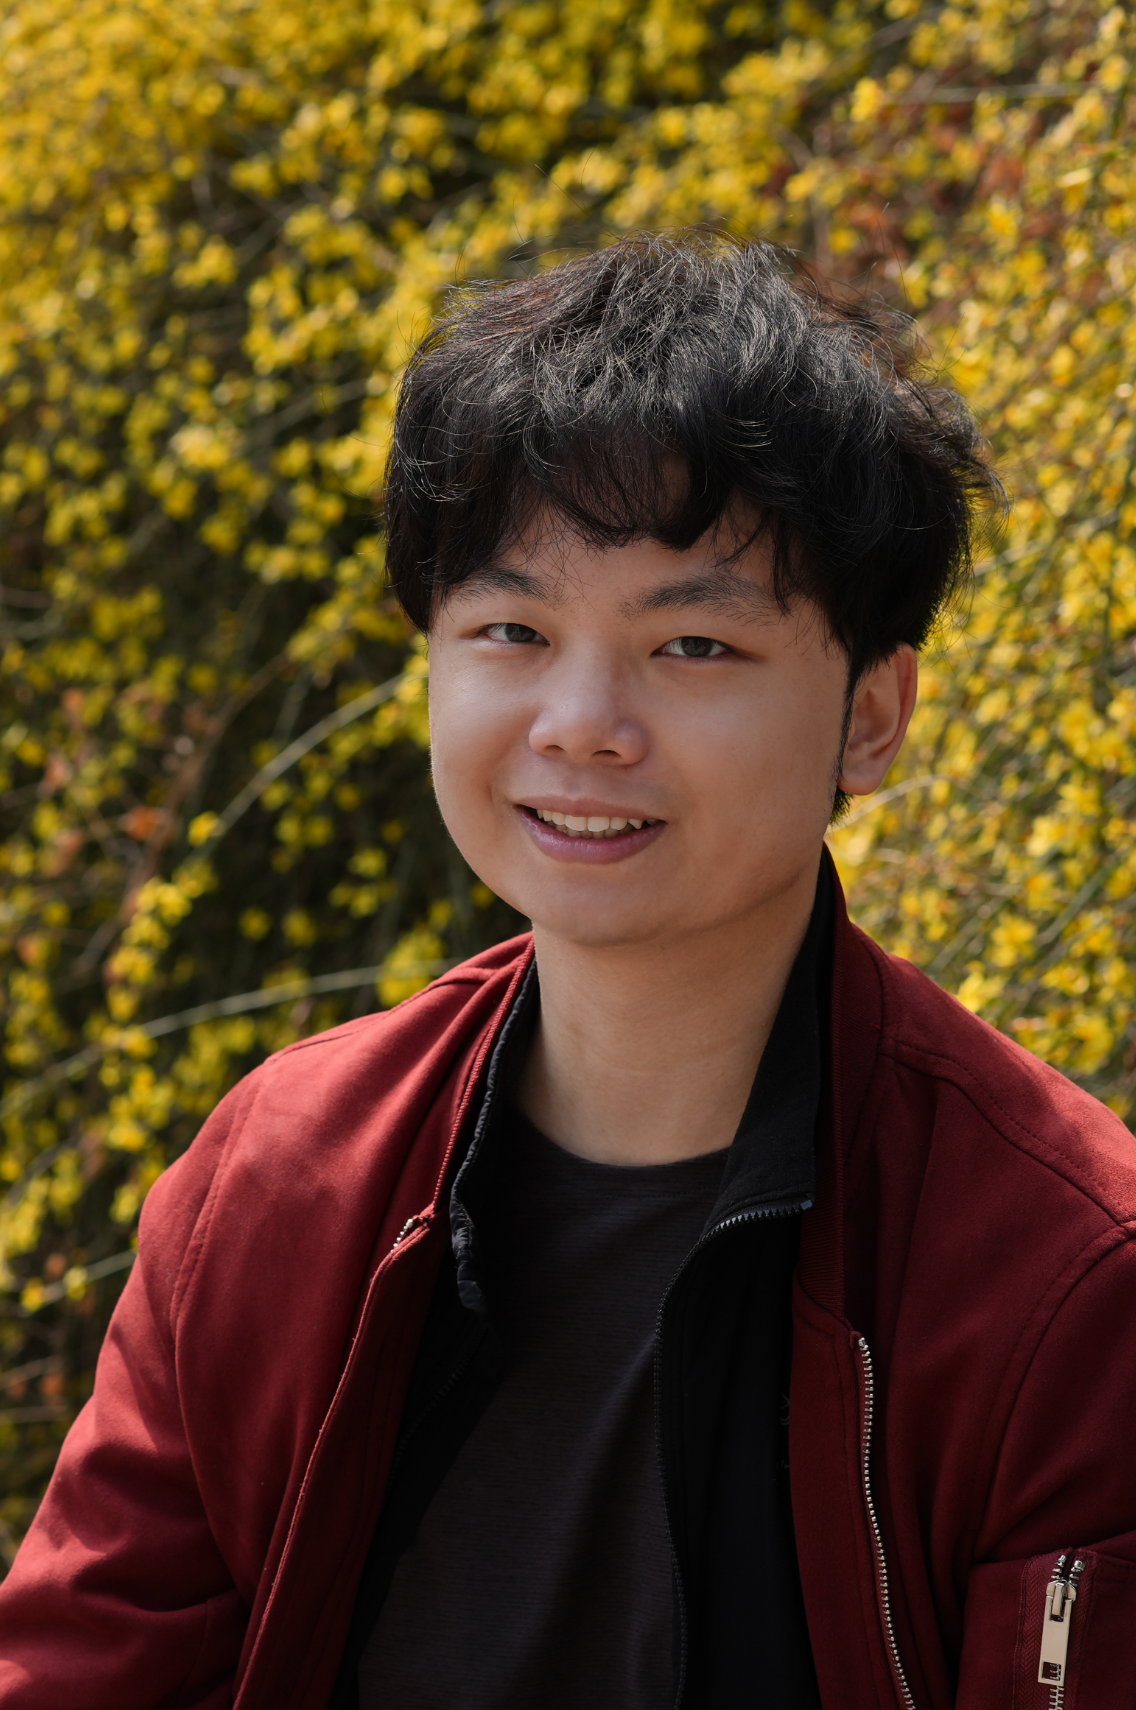
\includegraphics[width=105pt]{cv_photo} % 右侧图片
\end{minipage}

%-----------EDUCATION-----------------
    \cvsection{Education}{教育经历}{university}

    \cvsubHeadingListStart
    \lang{
        \cvsubheading
        {University of Cambridge}{}
        {Cambridge, UK}
        {Advanced Computer Science, Master of Philosophy (Distinction, Rank: 8/60)}{}
        {Oct 2024 --- Jul 2025}
    }{
        \cvsubheading
        {剑桥大学 | University of Cambridge}{}
        {剑桥，英国}
        {高级计算机科学，哲学硕士 （MPhil），杰出学位，排名：8/60}{}
        {2024年10月 --- 2025年7月}
    }
    \cvitemListStart
%    \cvitem
%    {Awarded Highly Commended M.Phil Project Prize 2024-2025 by the Department of Computer Science and Technology}
%    {获得剑桥大学计算机科学与技术系2024-2025年度硕士项目高度表彰奖（Highly Commended M.Phil Project Prize）}
    \cvitem
    {Courses: Geometric Deep Learning, Affective AI, Mobile \& Wearable ML, NLP, Multi-agent RL}
    {课程：几何深度学习，情感人工智能，移动与可穿戴设备机器学习，自然语言处理，多智能体强化学习}
    \cvitemListEnd

    \dashedhline
    \lang{
        \cvsubheading
        {University College London}{}
        {London, UK}
        {Computer Science, Bachelor of Science (First Class Honors)}{}
        {Sep 2021 --- Jun 2024}
    }{
        \cvsubheading
        {伦敦大学学院 | University College London}{}
        {伦敦，英国}
        {计算机科学，科学学士（BSc）， 一等荣誉学位}{}
        {2021年9月 --- 2024年6月}
    }
    \cvitemListStart
    \cvitem
    {Main Courses: Machine Learning, Computer Vision, Reinforcement Learning, Mathematics \& Statistics, Software Engineering}
    {主要课程：机器学习，计算机视觉，强化学习，数学与统计学，软件工程}
    \cvitemListEnd
    \cvsubHeadingListEnd

     \cvsection{Research Experience}{研究经验}{microscope}

    \cvsubHeadingListStart
    \lang{
        \cvsubheading
        {Protein Substructure Alignment via Optimal Transport}
        {Shanghai Jiao Tong University}
        {Shanghai, China}
        {Research Assistant}
        {Supervisor: Prof. Pietro Li\`o \& Prof. Liang Hong}
        {Apr 2025 --- Sep 2025}
    }{
        \cvsubheading
        {基于最优传输的蛋白质子结构对齐}
        {上海交通大学}
        {上海，中国}
        {助理研究员}
        {导师：洪亮教授}
        {2025年4月 --- 现在}
    }
    \cvitemListStart
    \cvitem
    {Developed PLASMA, a module based on optimal transport that can be seamlessly added to any protein representation learning model with minimal training or even no training to enable fast and highly accurate identification of locally similar substructures. (\link{https://arxiv.org/abs/2510.11752}{Paper})}
    {开发了PLASMA，一个基于最优传输的可以无缝添加到任何蛋白质语言模型中的模块，只需对模块使用 400 个样本进行训练（无需微调语言模型）甚至不训练，就能实现对局部相似子结构的高精度识别，并且能生成一个对齐矩阵来标注相似部分的具体位置。}
    \cvitem
    {Completed extensive experiments on 7 backbone protein language models across 3 tasks from the VenusX dataset (motifs, active sites, and binding sites), demonstrated consistant and significant improvement (+10-30\% ROC-AUC) across all backbones and tasks.}
    {在VenusX数据集的3个任务（基序、活性位点和结合位点）上对7个主干蛋白质语言模型进行了广泛实验，在所有主干模型和任务上都表现出一致且显著的改进（+10-30\% ROC-AUC）。}
    \cvitem
    {Conducted case studies using PyMol visualizations and proved that the founded similar substructures are indeed similar in structure and they are not found just because of sequence similarity.}
    {使用PyMol可视化进行案例研究，证明了所找到的相似子结构在结构上确实相似，并且不是仅仅因为序列相似性而被发现的。}
    \cvitemListEnd

    \dashedhline
    \lang{
        \cvsubheading
        {Hierarchical Protein Representation Learning}
        {University of Cambridge}
        {Cambridge, UK}
        {Research Assistant}
        {Supervisor: Prof. Pietro Li\`o}
        {Oct 2024 --- Sep 2025}
    }{
        \cvsubheading
        {基于拓扑神经网络的蛋白质结构表示学习}
        {剑桥大学}
        {剑桥，英国}
        {助理研究员}
        {导师：Pietro Li\`o教授}
        {2024年10月 --- 现在}
    }
    \cvitemListStart
%    \cvitem{
%    Invited by Prof. Liò to present this work at the University of Cambridge's Foundation AI Lecture Series. The talk is officially archived: \href{https://talks.cam.ac.uk/talk/index/234460}{talks.cam.ac.uk/talk/index/234460}. Paper: \href{https://arxiv.org/abs/2509.03885}{arxiv.org/abs/2509.03885}.
%    }
%    {
%    受 Liò 教授的邀请，在剑桥大学的 Foundation AI 演说系列中分享该工作。该演讲已被官方收录 \href{https://talks.cam.ac.uk/talk/index/234460}{talks.cam.ac.uk/talk/index/234460}。
%    }
    \cvitem
    {Developed TCPNet, an SE(3)-equivariant topological neural network that simultaneously learns protein residue-level and secondary structure-level features without losing any geometric information. (\link{https://talks.cam.ac.uk/talk/index/234460}{Invited Talk}) (\link{https://arxiv.org/abs/2509.03885}{Paper})}
    {开发了基于拓扑神经网络的 SE(3)-equivariant 蛋白质结构表示学习模型 TCPNet，可以同时学习蛋白质残基以及二级结构的特征，并保留所有的几何特征。}
    \cvitem{Awarded Highly Commended M.Phil Project Prize 2024-2025 by the Department of Computer Science and Technology}{}
    \cvitem{
    Demonstrated 5\% improvement on average across 3 popular protein representation learning tasks when only structure features are provided, which can be particularly important for de novo antibody design.
    }{
    当只提供结构信息时，实现了在 3 个蛋白质表示学习的任务上平均 5\% 的性能提升，体现了在从头抗体设计任务中的潜力。
    }
%    \cvitem
%    {Built a complete and extensible protein structure learning framework, including downloading raw PDB data, preprocessing into \texttt{combinatorial complexes} data structure, and computing features for various structural levels.}
%    {搭建了完整且易拓展的蛋白质结构学习框架，包含了原始 PDB 数据的下载、预处理为\texttt{combinatorial complexes}数据结构、各级结构的特征计算。}
%    \cvitem
%    {Refactored \texttt{TopoX}'s neighborhood matrix calculation to pure PyTorch, preventing GPU $\rightarrow$ CPU $\rightarrow$ GPU overhead and improving GPU utlization from 15\% to 50\% and shorten training time from 380 min to 90 min.}
%    {将 \texttt{TopoX} 库的 \texttt{combinatorial complex} 针对蛋白质结构重构为纯 PyTorch，实现了全流程 GPU 计算，避免了 GPU $\rightarrow$ CPU $\rightarrow$ GPU 的数据传输开销，将 GPU 利用率从 15\% 提升至 50\%并将训练时间缩短至四分之一。}
%    \cvitem
%    {Performed remote development on a \texttt{Linux HPC} server (with 4 A100 GPUs) using \texttt{SLURM} for job queuing and \texttt{WandB} for monitoring.}
%    {在\texttt{Linux HPC}服务器上（使用至多 4 个 A100 GPU）进行远程开发，使用\texttt{SLURM}进行作业排队，并利用\texttt{WandB}追踪实验进展。}
    \cvitemListEnd

    \dashedhline
    \lang{
        \cvsubheading
        {Multi-Omics Integration Data with GNNs}
        {University of Cambridge}
        {Cambridge, UK}
        {Research Assistant}
        {Supervisor: Prof. Pietro Li\`o}
        {Feb 2025 --- Sep 2025}
    }{
        \cvsubheading
        {基于 GNN 的多组学数据整合}
        {剑桥大学}
        {剑桥，英国}
        {助理研究员}
        {导师：Pietro Li\`o教授}
        {2025年2月 --- 现在}
    }
    \cvitemListStart
    \cvitem
    {Using heterogeneous graph network for embedding single cell multi-omics (e.g. RNA, protein, and ATAC modalities) data to a shared latent space and conduct cell clustering. (\link{https://arxiv.org/abs/2510.06880}{Paper})}
    {提出了一个基于 GAT 的轻量异构图神经网络，可以将单个细胞多模态序列分析数据（如 RNA、ADT和 ATAC）嵌入到共享的特征空间并做细胞聚类分析。}
    \cvitem
    {Training time on BM-CITE and LUNG-CITE datasets takes less than an hour on a laptop GPU, with 3\% lower ARI and 2\% lower NMI compared to the statistical method MOJITOO.}
    {在 BM-CITE 和 LUNG-CITE 数据集上的训练时间仅需几分钟（RTX 4070 GPU），相比纯统计的方法 MOJITOO 降低了 3\% 的 ARI，2\% 的 NMI。}
%    \cvitem
%    {Developed a pipeline with Python and R for downloading scRNA/ADT/ATAC-seq datasets stored in SeuratObject format and converting them to Python-readable AnnData.}
%    {用Python和R开发了完整的数据集下载以及预处理流程，用于下载以SeuratObject格式存储的scRNA/ADT/ATAC-seq数据，并转换为Python可读的AnnData格式。}
    \cvitemListEnd

    \dashedhline
    \lang{
        \cvsubheading
        {Graph-based Pain Estimation from Facial Expresissions}
        {University of Cambridge}
        {Cambridge, UK}
        {Research Assistant}
        {Supervisor: Prof. Hatice Gunes}
        {Oct 2024 --- Jan 2025}
    }{
        \cvsubheading
        {基于 GNN 的面部动作单元表示在疼痛强度估计中的应用}
        {剑桥大学}
        {剑桥，英国}
        {助理研究员}
        {导师：Hatice Gunes教授}
        {2024年10月 --- 2025年1月}
    }
    \cvitemListStart
    \cvitem
    {Presented at IJCAI25 MiGA Workshop. (\link{https://arxiv.org/abs/2505.19802v2}{Paper})}
    {独立一作论文被接收于 IJCAI25 MiGA Workshop。(\href{https://arxiv.org/abs/2505.19802v2}{arxiv.org/abs/2505.19802v2})}
    \cvitem
    {Proposed the GraphAU-Pain model that fuses a ResNet-50 backbone with graph-based facial action unit (AU) representation learning for pain intensity estimation, allowing better clinical interpretability and generalization compared to purely image-driven methods.}
    {提出了GraphAU-Pain模型，该模型使用了ResNet-50作为主干网络并融合了基于图神经网络的面部动作单元的表示学习用于疼痛强度估计，与纯图像特征驱动的方法相比具有更好的临床可解释性和泛化性。}
%    \cvitem
%    {Outperformed the state-of-art method GLA-CNN by 39\% in accuracy and 7\% in average F1-score when evaluating on the UNBC dataset.}
%    {在UNBC数据集上评估时，准确率比最先进的GLA-CNN方法提高了39\%，平均F1分数提高了7\%。}
    \cvitem
    {Developed a novel transfer learning strategy to address domain differences and missing annotations, improving GraphAU-Pain's AU occurrence prediction F1-score by 30\% on the UNBC dataset.}
    {提出了一种新的迁移学习策略以解决领域差异和缺失标注问题，使GraphAU-Pain模型在UNBC数据集上AU出现预测的F1分数提高了30\%。}
    \cvitemListEnd

    \newpage
%    \dashedhline
    \lang{
        \cvsubheading
        {Readmission Prediction with Remote Patient Monitoring Data}
        {University College London}
        {London, UK}
        {Research Assistant}
        {Supervisor: Prof. Ivana Drobnjak}
        {May 2023 --- Jun 2024}
    }{
        \cvsubheading
        {RPM手术并发症预测模型}
        {伦敦大学学院}
        {伦敦，英国}
        {助理研究员}
        {导师：Ivana Drobnjak教授}
        {2023年5月 --- 2024年6月}
    }
    \cvitemListStart
    \cvitem
    {Collaborated with clinicians from UCL Hospital to develop a SQL-based data pipeline for processing raw remote patient monitoring data, performing clinical feature engineering, and building interpretable ML models (ROC-AUC 0.79±0.03) with \texttt{SHAP} analysis.}
    {与UCL医院临床医生合作，开发基于\texttt{PostgreSQL}的数据流水线处理原始远程患者监测数据，进行临床特征工程，并构建可解释的机器学习模型（ROC-AUC 0.79±0.03），使用\texttt{SHAP}进行分析。}

    \cvitem
    {Designed a patient-independent stratified bootstrapping evaluation framework to address extreme data scarcity (55 patients) and class imbalance, preventing data leakage and ensuring robust generalization estimates for clinical deployment.}
    {设计了患者独立的分层自助法评估框架，以应对极端数据稀缺（55名患者）和类别不平衡问题，防止数据泄露并确保临床部署的稳健泛化估计。}
    \cvitemListEnd
    \cvsubHeadingListEnd

%-----------INDUSTRIAL EXPERIENCE-----------------
    \cvsection{Industrial Experience}{行业经验}{briefcase}

    \cvsubHeadingListStart
    \lang{
        \cvsubheading
        {Hierarchical Reasoning Model for Healthcare}
        {Sapient Intelligence}
        {Beijing, China}
        {AI Research \& Application Engineer}
        {}
        {Sep 2025 --- Present}
    }{
        \cvsubheading
        {基于合成数据生成的医疗LLM知识蒸馏}
        {科大讯飞医疗健康技术有限公司}
        {合肥, 中国}
        {助理研究算法工程师}
        {导师：蔡健宇}
        {2024年7月 --- 2024年9月}
    }
    \cvitemListStart
    \cvitem
    {Applying \link{https://github.com/sapientinc/HRM}{Hierarchical Reasoning Models} to healthcare scenarios and collaborating with Peking Union Medical College Hospital to develop healthcare solutions.}
    {开发了知识蒸馏流水线，利用通用教师LLM从10个人工标注样本中合成1000+医疗指令遵循样例，将学生模型在医疗特定指令上的任务完成准确率从34\%提升至82\%。}
    \cvitemListEnd

    \dashedhline
    \lang{
        \cvsubheading
        {Healthcare LLM Knowledge Distillation}
        {Xunfei Healthcare Technology}
        {Hefei, China}
        {Assistant AI Research Engineer}
        {}
        {Jul 2024 --- Sep 2024}
    }{
        \cvsubheading
        {基于合成数据生成的医疗LLM知识蒸馏}
        {科大讯飞医疗健康技术有限公司}
        {合肥, 中国}
        {助理研究算法工程师}
        {导师：蔡健宇}
        {2024年7月 --- 2024年9月}
    }
    \cvitemListStart
    \cvitem
    {Built a knowledge distillation pipeline using a teacher LLM to synthesize medical instruction examples from human-annotated samples, improving student model (\link{https://www.xunfeihealthcare.com/en/product/244.html}{Xiaoyi}) instruction-following accuracy from 34\% to 82\% via supervised fine-tuning.}
    {开发了知识蒸馏流水线，利用通用教师LLM从10个人工标注样本中合成1000+医疗指令遵循样例，将学生模型在医疗特定指令上的任务完成准确率从34\%提升至82\%。}
%    \cvitem
%    {Enhanced instruction generation methods, extending short general instructions (10–50 words) to domain-specific ones averaging 500 words for advanced healthcare-specific LLM training.}
%    {改进了指令生成方法，将简短（10–50字）的通用指令扩展到平均500字的领域特定指令，针对医疗专用 LLM 的训练。}
%    \cvitem
%    {Ensured synthetic data diversity using a two-layer algorithm: the first layer generated structured instructions of varying difficulty, and the second rewrote them into diverse forms.}
%    {采用两层算法确保合成数据的多样性：第一层生成难度各异的结构化指令，第二层将其改写成多种形式。}
%    \cvitem
%    {Used an iterative output generation algorithm for instruction–input pairs to improve the LLM's output accuracy from 72\% to 91\%.}
%    {开发了一个指令和输入进行迭代输出生成算法，将LLM输出准确率在15次迭代中从72\%提升至91\%。}
    \cvitemListEnd

    \dashedhline
    \lang{
        \cvsubheading
        {RAG-Based Financial Intelligence System}
        {Luojin Data Information}
        {Shanghai, China}
        {Intern Machine Learning Engineer}
        {}
        {May 2023 --- Aug 2023}
    }{
        \cvsubheading
        {基于RAG的金融智能系统}
        {上海珞瑾数据有限公司}
        {上海, 中国}
        {实习算法工程师}
        {}
        {2023年5月 --- 2023年8月}
    }
    \cvitemListStart
    \cvitem
    {Developed a Retrieval-Augmented Generation (RAG) pipeline with \texttt{MongoDB} vector store and \texttt{LangChain} agents for automated financial report classification, achieving 92\% query translation accuracy and 97\% entity matching rate through semantic search.}
    {开发了基于检索增强生成（RAG）的流水线，使用\texttt{MongoDB}向量存储和\texttt{LangChain}代理实现财务报告自动分类，通过语义搜索达到92\%的查询转换准确率和97\%的实体匹配率。}
    \cvitemListEnd

    \dashedhline
    \lang{
        \cvsubheading
        {Low-cost AI Chatbot Generation System for Hospitals}
        {National Health Service}
        {London, UK}
        {Intern Software Engineer}
        {}
        {Sep 2022 --- May 2023}
    }{
        \cvsubheading
        {低成本医院AI聊天机器人生成系统}
        {英国国民健康署}
        {伦敦，英国}
        {实习软件工程师}
        {}
        {2022年9月 --- 2023年5月}
    }
    \cvitemListStart
    \cvitem
    {Created an automated chatbot generation service for hospitals, reducing development time from weeks to 30 minutes.}
    {带领3人团队使用\texttt{React.js}和\texttt{Django}开发了一个医院自动生成聊天机器人的服务，将开发时间从数周缩短到30分钟。}
    \cvitem
    {Delivered a live demonstration at Great Ormond Street Hospital to clinicians, and presented at UCL to IBM, Microsoft, and Intel, earning \link{https://bit.ly/ixn-nhs-ucl-and-ibm}{media recognition} from an IBM Master Inventor.}
    {在Great Ormond Street Hospital进行现场演示，并在UCL向IBM、Microsoft和Intel展示，获得IBM Master Inventor John McNamara的博客报道。（\link{https://bit.ly/ixn-nhs-ucl-and-ibm}{bit.ly/ixn-nhs-ucl-and-ibm}）。}

%    \cvitem
%    {Deployed a \texttt{Scrapy} web crawler to extract key hospital information and formatted it into Q\&A pairs.}
%    {部署了\texttt{Scrapy}网络爬虫，从医院主页提取关键信息，并将其格式化为问答对。}
%    \cvitem
%    {Engineered a multi-layer Q\&A architecture that reduced service costs by 50\% and improved answer accuracy by 20\%.}
%    {设计了多层问答架构，将服务成本降低50\%并提高答案准确率20\%。}
    \cvitemListEnd



    \cvsubHeadingListEnd

%-----------TEACHING EXPERIENCE-----------------
%    \cvsection{Teaching Experience}{教学经验}



%-----------ADDITIONAL EXPERIENCE-----------------
    \cvsection{Additional Experience}{其他经历}{thumbtack}

    \cvsubHeadingListStart


%    \dashedhline
    \lang{
        \cvsubheading
        {Fresher Coding Sessions}
        {University College London}
        {London, UK}
        {Programming Tutor}
        {}
        {Sep 2022 --- May 2023}
    }{
        \cvsubheading
        {新生编程辅导}
        {伦敦大学学院}
        {伦敦，英国}
        {编程辅导员}
        {}
        {2022年9月 --- 2023年5月}
    }
    \cvitemListStart
    \cvitem
    {Organized biweekly group discussions for 12 first-year computer science students, offering academic guidance and peer support.}
    {为12名大一计算机科学学生每两周组织小组讨论，提供学术指导和同伴支持。}
%    \cvitem
%    {Delivered targeted lessons using examples from my first-year assignments, earning excellent feedback.}
%    {利用大一作业中的实例讲授课程，获得了优秀反馈。}
    \cvitemListEnd
    \cvsubHeadingListEnd

%-----------OTHER INFORMATION-----------------
%    \cvsection{Other Information}{其他信息}{sticky-note}
%
%    \cvsubHeadingListStart
%    \cvitem
%    {\textbf{Programming Languages:} Python, JavaScript, Java, Typescript, C++, C, R}
%    {编程语言：Python, JavaScript, Java, Typescript, C++, C, R}
%    \cvitem
%    {\textbf{AI Libraries:} PyTorch, PyTorch Lightning, PyTorch Geometric, Numpy, Pandas, Scikit-Learn}
%    {AI库：PyTorch, PyTorch Lightning, PyTorch Geometric, Numpy, Pandas, Scikit-Learn}
%    \cvitem
%    {\textbf{Visualization Libraries:} Matplotlib, Seaborn, Plotly}
%    {可视化库：Matplotlib, Seaborn, Plotly}
%%    \cvitem
%%    {Visa Status: Student Visa (until Aug 2025), but will apply for a Graduate Visa after graduation, which permits full-time working for 2 years. No need for sponsorship.}
%%    {}
%    \cvsubHeadingListEnd

\end{document}
